% Digital Logic Report Template
% Created: 2020-01-10, John Miller

%==========================================================
%=========== Document Setup  ==============================

% Formatting defined by class file
\documentclass[11pt]{article}

% ---- Document formatting ----
\usepackage[margin=1in]{geometry}	% Narrower margins
\usepackage{booktabs}				% Nice formatting of tables
\usepackage{graphicx}				% Ability to include graphics

%\setlength\parindent{0pt}	% Do not indent first line of paragraphs 
\usepackage[parfill]{parskip}		% Line space b/w paragraphs
%	parfill option prevents last line of pgrph from being fully justified

% Parskip package adds too much space around titles, fix with this
\RequirePackage{titlesec}
\titlespacing\section{0pt}{8pt plus 4pt minus 2pt}{3pt plus 2pt minus 2pt}
\titlespacing\subsection{0pt}{4pt plus 4pt minus 2pt}{-2pt plus 2pt minus 2pt}
\titlespacing\subsubsection{0pt}{2pt plus 4pt minus 2pt}{-6pt plus 2pt minus 2pt}

% ---- Hyperlinks ----
\usepackage[colorlinks=true,urlcolor=blue]{hyperref}	% For URL's. Automatically links internal references.

% ---- Code listings ----
\usepackage{listings} 					% Nice code layout and inclusion
\usepackage[usenames,dvipsnames]{xcolor}	% Colors (needs to be defined before using colors)

% Define custom colors for listings
\definecolor{listinggray}{gray}{0.98}		% Listings background color
\definecolor{rulegray}{gray}{0.7}			% Listings rule/frame color

% Style for Verilog
\lstdefinestyle{Verilog}{
	language=Verilog,					% Verilog
	backgroundcolor=\color{listinggray},	% light gray background
	rulecolor=\color{blue}, 			% blue frame lines
	frame=tb,							% lines above & below
	linewidth=\columnwidth, 			% set line width
	basicstyle=\small\ttfamily,	% basic font style that is used for the code	
	breaklines=true, 					% allow breaking across columns/pages
	tabsize=3,							% set tab size
	commentstyle=\color{gray},	% comments in italic 
	stringstyle=\upshape,				% strings are printed in normal font
	showspaces=false,					% don't underscore spaces
}

% How to use: \Verilog[listing_options]{file}
\newcommand{\Verilog}[2][]{%
	\lstinputlisting[style=Verilog,#1]{#2}
}




%======================================================
%=========== Body  ====================================
\begin{document}

\title{ELC 2137 Lab \#7: Binary Coded Decimal}
\author{Sean Dickenscheidt and Sebastion Lopez}

\maketitle


\section*{Summary}

In this lab, the basic of Verilog were learned. It was discovered how to create a half-adder, full-adder, and 
an adder/subtractor. The more complited the circuit, the more things it can do.


\section*{Results}


\begin{lstlisting}[style=Verilog,
caption=Add3 code,
label=code:ex 
]
`timescale 1ns / 1ps
// ELC 2137 - Lab6 - 02/20/2020
// Sebastian Lopez and Sean Dickenscheidt 

module add3 (
input [3:0] in, 
output reg [3:0] out
);

always @* 
begin
if (in >= 5)
out = in + 3; 
else
out = in;
end  

endmodule //add3
\end{lstlisting}

\begin{lstlisting}[style=Verilog,
caption=BCD6 code,
label=code:ex 
]
`timescale 1ns / 1ps
// ELC 2137 - Lab6 - 02/20/2020
// Sebastian Lopez and Sean Dickenscheidt 

module BCD6 (
input [5:0] B, 
output reg [7:0] Output6
);

wire w1, w2, w3, w4, w5, w6;

assign Output6[7] = 0; 
assign Output6[0] = B[0];

add3 Bobby(
.in({1'b0, B[5:3]}), 
.out({Output6[6], w1, w2, w3}) 
);
add3 Billy(
.in({w1, w2, w3, B[2]}), 
.out({Output6[5], w4, w5, w6})
);
add3 Barron(
.in({w4, w5, w6, B[1]}),
.out({Output6[4], Output6[3], Output6[2], Output6[1]})
);

endmodule //BCD 6


\end{lstlisting}

\begin{lstlisting}[style=Verilog,
caption=BCD11 code,
label=code:ex 
]
`timescale 1ns / 1ps
// ELC 2137 - Lab6 - 02/20/2020
// Sebastian Lopez and Sean Dickenscheidt 

module BCD11 (
input [10:0] B, 
output [13:0] Output11 
);

wire w1, w2, w3, w4, w5, w6, w7, w8, w9, w10;
wire w11, w12, w13, w14, w15, w16, w17, w18, w19, w20;
wire w21, w22, w23, w24, w25, w26, w27, w28, w29, w30;
wire w31, w32, w33, w34, w35, w36, w37, w38, w39, w40;
wire w41, w42, w43, w44, w45, w46, w47;

assign Output11[0] = B[0];

add3 Bobby(
.in({1'b0, B[10:8]}), 
.out({w1, w2, w3, w4}) 
);
add3 Billy(
.in({w2, w3, w4, B[7]}), 
.out({w5, w6, w7, w8})
);
add3 Barron(
.in({w6, w7, w8, B[6]}),
.out({w9, w10, w11, w12})
);
add3 Barry(
.in({1'b0, w1, w5, w9}),
.out({w13, w14, w15, w16})
);
add3 Bart(
.in({w10, w11, w12, B[5]}),
.out({w17, w18, w19, w20})
);
add3 Blake(
.in({w14, w15, w16, w17}),
.out({w21, w22, w23, w24})
);
add3 Ben(
.in({w18, w19, w20, B[4]}),
.out({w25, w26, w27, w28})
);
add3 Brody(
.in({w22, w23, w24, w25}),
.out({w29, w30, w31, w32})
);
add3 Brett(
.in({w26, w27, w28, B[3]}),
.out({w33, w34, w35, w36})
);
add3 Sebas(
.in({1'b0, w13, w21, w29}),
.out({Output11[13], w37, w38, w39})
);
add3 Sean(
.in({w30, w31, w32, w33}),
.out({w40, w41, w42, w43})
);
add3 Steve(
.in({w34, w35, w36, B[2]}),
.out({w44, w45, w46, w47})
);
add3 Shane(
.in({w37, w38, w39, w40}),
.out({Output11[12], Output11[11], Output11[10], Output11[9]})
);
add3 Sam(
.in({w41, w42, w43, w44}),
.out({Output11[8], Output11[7], Output11[6], Output11[5]})
);
add3 Seth(
.in({w45, w46, w47, B[1]}),
.out({Output11[4], Output11[3], Output11[2], Output11[1]})
);

endmodule //BCD 11
\end{lstlisting}

\begin{lstlisting}[style=Verilog,
caption=sseg1 code,
label=code:ex 
]
`timescale 1ns / 1ps
// ELC 2137 - Lab6 - 02/20/2020
// Sebastian Lopez and Sean Dickenscheidt 

module sseg1_BCD  (
input [15:0] sw, 
output [3:0] an, 
output [6:0] seg, 
output dp
); 
wire [13:0] sseg1_wire; 
wire [1:0] thousands; 
wire [3:0] hundreds, tens, ones; 
wire [3:0] out1; 

BCD11 sseg1(
.B(sw[10:0]),
.Output11(sseg1_wire)
);

assign thousands = sseg1_wire[13:12]; 
assign hundreds = sseg1_wire[11:8]; 
assign tens = sseg1_wire[7:4]; 
assign ones = sseg1_wire[3:0];

mux2_4b Test1(
.in0(ones), .in1(tens), .sel(sw[15]),
.out(out1)
);  

sseg_decoder Test2(
.num(out1), 
.sseg(seg)
);

assign an[1] = sw[15]; 
assign an[0] = sw[15]; 
assign an[3:2] = 2'b11; 
assign dp = 1;   

endmodule //sseg1_BCD
\end{lstlisting}

\begin{lstlisting}[style=Verilog,
caption=Add3 test code,
label=code:ex 
]
`timescale 1ns / 1ps
// ELC 2137 - Lab6 - 02/20/2020
// Sebastian Lopez and Sean Dickenscheidt 

module add3_test ();

reg [3:0] in;
wire [3:0] out;

integer i; 

add3 Bobby(
.in(in), 
.out(out)
);

initial 
begin 

for (i =0; i <= 4'b1111; i = i + 1)
begin 
in = i;
#10;
end 

$finish;

end 
endmodule //add3_test


\end{lstlisting}

\begin{lstlisting}[style=Verilog,
caption=BCD6 test code,
label=code:ex 
]
`timescale 1ns / 1ps
// ELC 2137 - Lab6 - 02/20/2020
// Sebastian Lopez and Sean Dickenscheidt 

module BCD6_test ();

reg [5:0] B; 
wire [7:0] Output6;

integer i; 

BCD6 test1( 
.B(B), 
.Output6(Output6)
);

initial 
begin 

for (i =0; i <= 6'b111111; i = i + 1)
begin 
B = i;
#10;
end 

$finish;

end 

endmodule //BCD6_Test
\end{lstlisting}

\begin{lstlisting}[style=Verilog,
caption=BCD11 test code,
label=code:ex 
]
`timescale 1ns / 1ps
// ELC 2137 - Lab6 - 02/20/2020
// Sebastian Lopez and Sean Dickenscheidt 

module BCD11_test ();

reg [10:0] B; 
wire [13:0] Output11;

integer i; 

BCD11 test1( 
.B(B), 
.Output11(Output11)
);

initial 
begin 

for (i =0; i <= 11'b11111111111; i = i + 1)
begin 
B = i;
#10;
end 

$finish;

end 

endmodule //BCD11_Test
\end{lstlisting}



	\begin{figure}[ht]\centering
		
		
		
		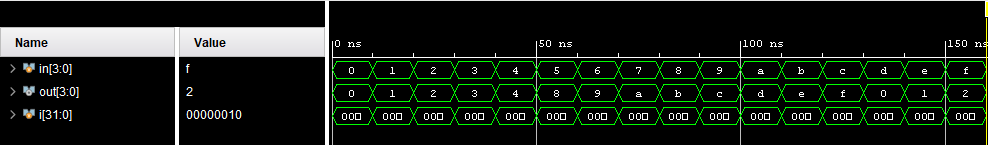
\includegraphics[width=1\textwidth,angle=0,origin=c]{add3_test.PNG}
		\caption{Add3}
		\label{fig:sim_with_table}
		
	\end{figure}

	\begin{figure}[ht]\centering
		
		
		
		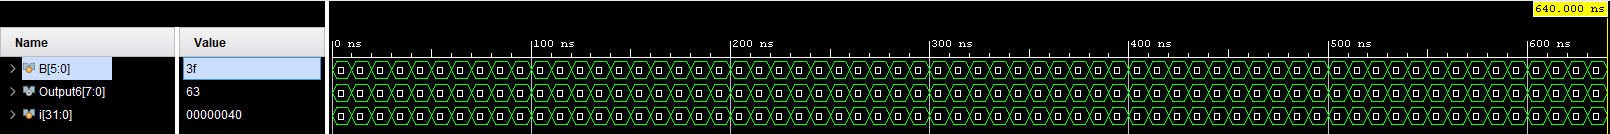
\includegraphics[width=1\textwidth,angle=0,origin=c]{BCD6_test.PNG}
		\caption{BCD6}
		\label{fig:sim_with_table}
		
	\end{figure}
	
	

	
	\begin{figure}[ht]\centering
		
		
		
		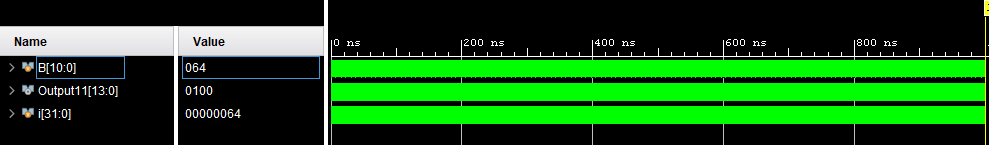
\includegraphics[width=1\textwidth,angle=0,origin=c]{BCD11.PNG}
		\caption{BCD11}
		\label{fig:sim_with_table}
		
	\end{figure}


\begin{figure}[ht]\centering
	
	
	
	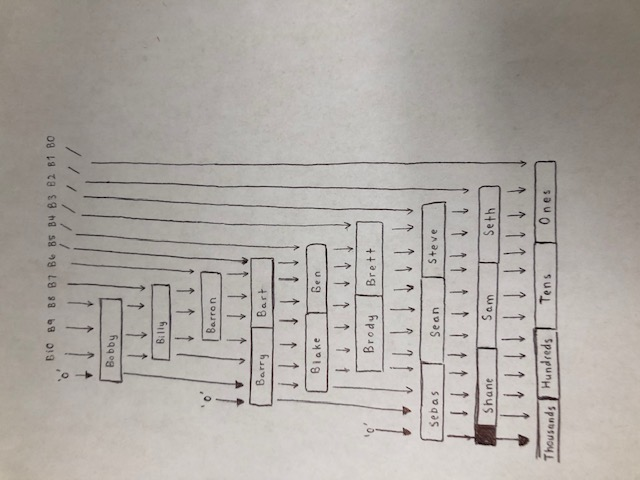
\includegraphics[width=1\textwidth,angle=270,origin=c,scale=1]{bcd11.jpg}
	\caption{BCD11}
	\label{fig:sim_with_table}
	
\end{figure}
	
	
\end{document}
